\documentclass{article}

% NeurIPS style: 9 pages of main text (plus references and appendix).
% `preprint` shows author names; use \usepackage{neurips_2025} alone for an anonymous submission.
\usepackage[preprint]{neurips_2025}

\usepackage[utf8]{inputenc}
\usepackage[T1]{fontenc}
\usepackage{hyperref}
\usepackage{url}
\usepackage{booktabs}
\usepackage{amsfonts,amsmath,amssymb,amsthm}
\usepackage{nicefrac}
\usepackage{microtype}
\usepackage{xcolor}
\usepackage{graphicx}
\usepackage{subcaption}
\usepackage{multirow}
\usepackage{listings}
\usepackage{tikz}
\usetikzlibrary{arrows.meta,positioning,fit,calc,shapes.misc}
\usepackage{pgfplots}
\pgfplotsset{compat=1.18}
\usepackage[capitalize,noabbrev]{cleveref}

\hypersetup{colorlinks=true,linkcolor=blue!50!black,citecolor=blue!50!black,urlcolor=blue!50!black}

\theoremstyle{plain}
\newtheorem{theorem}{Theorem}
\newtheorem{proposition}{Proposition}
\newtheorem{corollary}{Corollary}
\theoremstyle{definition}
\newtheorem{definition}{Definition}
\theoremstyle{remark}
\newtheorem{remark}{Remark}

\lstdefinelanguage{nerve}{
  morekeywords={nerve,name,state,actions,transitions,invariants,ensures,futures,learn,initial,when,type,range,values,params,kind,over,after,holds,fallback,examples,action,next},
  sensitive=true, morecomment=[l]{\#}, morestring=[b]", morestring=[b]'
}
\lstset{language=nerve,basicstyle=\ttfamily\scriptsize,keywordstyle=\bfseries,commentstyle=\color{gray},
  columns=fullflexible,keepspaces=true,breaklines=true,frame=single,framerule=0.3pt,xleftmargin=4pt,xrightmargin=4pt,aboveskip=4pt,belowskip=4pt}

\newcommand{\method}{\textsc{Nerve}\xspace}
\usepackage{xspace}
\newcommand{\Sset}{\mathcal{S}}
\newcommand{\Aset}{\mathcal{A}}
\newcommand{\onehot}{\operatorname{onehot}}
\newcommand{\relu}{\operatorname{relu}}
\newcommand{\dH}{d_{\mathrm{H}}}
\newcommand{\Ec}{E_{\mathrm{c}}}
\newcommand{\Ej}{E_{\mathrm{J}}}
\newcommand{\Ef}{E_{\mathrm{F}}}
\newcommand{\Eth}{E_{\theta}}
\newcommand{\bz}{\mathbf{z}}
\newcommand{\bx}{\mathbf{x}}
\newcommand{\be}{\mathbf{e}}
\newcommand{\R}{\mathbb{R}}
\newcommand{\ind}[1]{\mathbb{1}[#1]}

\newcommand{\mainsummary}{On the CPU re-runs, counter (with hole) misses 1, 1, 0 of 34 held-out cells across seeds 0--2; slider (gridded) misses 0, 0, 1 of 213 held-out cells across seeds 0--2; negotiate is exact on all 367 held-out cells in all 3 seeds; in total 6 of 9 (spec, seed) runs are exact on every held-out cell, and no run produces a spec violation.}
\newcommand{\holesummary}{$1.00/1.00/1.00$ on the five examples, seeds 0--2}
\newcommand{\nofactheld}{100.0}
\newcommand{\ablatesummary}{Without the factored head, negotiation falls to 1.000/1.000/1.000 held-out exact (seeds 0--2) while seen cells stay at 1.000 overall; the slider falls to 0.991 and the counter to 0.941; removing the ordinal read-out as well gives 1.000, 0.991 and 0.971; with the factored head present, lowering weight decay to $10^{-4}$ gives 1.000, 1.000 and 0.971.}
\newcommand{\holdoutsummary}{negotiate: 1.000 at 15\% (367 cells), 1.000 at 30\% (741 cells), 1.000 at 50\% (1195 cells); slider: 1.000 at 15\% (213 cells), 0.998 at 30\% (449 cells), 0.999 at 50\% (731 cells); counter: 0.971 at 15\% (34 cells), 0.934 at 30\% (76 cells), 0.931 at 50\% (131 cells); without the factored head at 30\%: negotiate 1.000, slider 0.971, counter 0.882.}
\newcommand{\toggleparams}{96,196}
\newcommand{\counterparams}{111,212}
\newcommand{\sliderparams}{121,832}
\newcommand{\negparams}{140,018}
\newcommand{\counterH}{280}
\newcommand{\counterCparams}{15{,}680}
\newcommand{\negH}{2{,}376}
\newcommand{\negCparams}{225{,}720}
\newcommand{\negmarginmin}{74}
\newcommand{\negmarginmed}{93}
\newcommand{\negmarginminseen}{75}
\newcommand{\negspread}{1665}
\newcommand{\negcpu}{5.3}
\newcommand{\contexact}{99.8}
\newcommand{\contexactcpu}{0.915}
\newcommand{\contexactcpupct}{91.5}
\newcommand{\sweephours}{1.2}
\newcommand{\pulseonesparsity}{7.8\%}
\newcommand{\pulseonekb}{31}
\newcommand{\pulsesummary}{at the training learning rate ($3\times10^{-3}$, five epochs) 99\% of values change and the patch is 1.2$\times$ smaller than the checkpoint only through compression (\cref{tab:pulse}).}


\title{\method: Software Without Code\\
\large Compiling Behavior Specifications into Exact Weights and Training the Rest as an Energy}

\author{%
  Alex Welcing\\
  Lupine Science, Inc.\\
  \texttt{alexwelcing@gmail.com}\\
}

\begin{document}

\maketitle

\begin{abstract}
We ask what it takes to ship a small interactive program as a neural network that is held to its specification, rather than as code. \method takes a behavior spec---typed state, guarded pure transitions, invariants, post-conditions, the set of states a gesture may lead to, and \emph{holes} given only by examples---and produces a network that maps a state and a user action to the next state by minimizing an energy over candidate futures. The energy has three terms. Transitions the spec writes down are compiled, with no training, into a two-layer ReLU network whose energy is exactly the normalized Hamming distance to the true successor; it is silent on holes. An action-conditioned joint-embedding predictive architecture supplies prediction error as energy. A factored per-field head with a shift kernel indexed by the offset from the field's current value makes ``$+1$'' the same function at every value of the field. Trained with InfoNCE over all candidates and a hinge on spec-violating futures, the learned terms alone---the circuit disabled---match the oracle on every held-out (state, action) cell for seven finite interfaces of up to $404$ states $\times$ $103$ actions in the repository's runs, three of the interfaces specified from screenshots by a vision agent without hand edits; three-seed CPU re-runs of the four hand-written specs reproduce this on negotiation and the gridded slider and miss at most one boundary cell on the counter. A continuous slider reaches \contexact{}\% within tolerance by gradient descent on the energy in the repository's run (\contexactcpupct{}\% in our CPU re-run from the default log). Ablations locate the factored head's contribution: where a rule is a shift along an ordinal field it carries the held-out cells as the held-out fraction grows (slider with 30\% of cells held out: 436 of 449 without it, 448 with it; counter: 67 and 71 of 76), while the negotiation game, whose rules are absolute assignments, is recovered exactly from half of its transition table by the JEPA term alone. Conformance is measured on the BF16 weights that ship; a Cloudflare Worker and a browser execute the same network; continued training is shipped as bit-identical sparse weight patches; and an evolving team of coding agents produced the negotiation network for \$14.23. We also say plainly what this is not: the interfaces are small, the compiled circuit is a lookup table in weight form, and the generalization we measure is within an interface, not across interfaces.
\end{abstract}

\section{Introduction}
\label{sec:intro}

Software is a state machine: a state, a set of actions a user can take, a transition function, and properties that must hold before and after every step. We ship it as code. This paper asks what it takes to ship it as a network instead---not a model that \emph{writes} the program, but a network that \emph{is} the program, in the plain sense that it takes the interface's state and a user action and returns the next state, and is held to a specification the way code is held to types and tests.

Three things make the question worth asking now. First, a behavior specification is a smaller and more checkable artifact than an implementation, and the part of it that is explicit can be \emph{compiled} into weights rather than learned, so the network is exact where the spec is explicit and learning is spent only on what the spec can show but not write (ink-style holes~\citep{inklang}) and on cells it never saw. Second, a network's runtime is one function---a forward pass and an argmin---that runs identically on a GPU trainer, a CPU worker, an edge isolate, or a browser tab, and an update to it is a sparse weight patch, not a deployment. Third, recent work compiles exact computation into the weights of language models~\citep{qwenputer,qwengpu,cajal}, which suggests a future in which an interface compiled this way is a component other networks can hold.

\method is the smallest system we could build that takes this seriously end to end. The input is a \texttt{.nerve} spec (\cref{sec:spec}), written by hand or produced from code, prose, or a screenshot by an agent that iterates against the spec checker. The output is a network whose energy $E(s,a,s')$ over candidate next states $s'$ is a sum of three terms (\cref{sec:compile,sec:energy}): a \emph{compiled circuit}, exact by construction on every transition the spec writes down and constant elsewhere; a \emph{JEPA} term~\citep{lecun2022path,assran2023ijepa}, the squared prediction error of an action-conditioned predictor in representation space; and a \emph{factored per-field} term whose shift kernel is translation-equivariant along ordinal fields. Inference is $\arg\min_{s'} E$ over the states a gesture may lead to (the \emph{futures} of declarative dragging~\citep{dragology}), or gradient descent on $E$ for continuous fields. The network that ships is BF16; a Cloudflare Worker, Cloudflare's open-source \texttt{workerd}, and a static browser bundle execute the identical energy, and continued training reaches them as sparse patches that are verified bit-identical by digest (\cref{sec:ship}).

The repository this work lives in began as the end-to-end negotiator of \citet{lewis2017deal}: one network, one task, supervised then self-play. We keep a finite version of that negotiation game as one of our specs and change the question from \emph{can a network learn to negotiate} to \emph{can a network be held to the rules of the game}.

\paragraph{Contributions.}
(1)~A behavior-spec language with a mechanically derived reference interpreter and self-check, and an intake path from code, prose, or screenshots (\cref{sec:spec}).
(2)~An exact compiler from finite specs to ReLU weights, with a proof that the compiled energy equals the normalized Hamming distance to the true successor and a condition under which it dominates any learned term (\cref{sec:compile}).
(3)~An energy model that combines JEPA prediction error with a factored per-field head whose shift kernel is translation-equivariant along ordinal fields, and ablations that say where the head matters (shift rules, large hold-out) and where it does not (\cref{sec:energy,sec:results}).
(4)~An evaluation protocol for networks-as-programs: deterministic hold-out of (state, action) cells, learned-only scoring with the circuit disabled, violation rate against the spec, scores taken from the BF16 weights that ship, and runtime parity over HTTP (\cref{sec:protocol}).
(5)~Results on eight specs, three of them from screenshots; ablations and seed variance; continuous inference; sparse patching; and a case study of an evolving agent team (\cref{sec:results,sec:ship}).
Everything in this paper is one branch of one public repository and reproduces on a two-core CPU; the negotiation network trains in under five minutes.

\section{Behavior specifications}
\label{sec:spec}

\begin{figure}[t]
\centering
\begin{minipage}[t]{0.46\textwidth}
\begin{lstlisting}
nerve: 1
name: counter
state:
  count: {type: int, range: [0, 9]}
  armed: {type: bool}
actions:
  inc: {}
  dec: {}
  arm: {}
  set: {params: {to: {type: int, range: [0, 9]}}}
  nudge: {}      # behaviour given only by examples
transitions:
  inc: { when: "armed", count: "min(count + 1, 9)" }
  dec: { when: "armed", count: "max(count - 1, 0)" }
  arm: { armed: "not armed" }
  set: { count: "to" }
invariants: ["0 <= count <= 9"]
ensures:
  - { after: inc, holds: "count >= old.count" }
  - { after: set, holds: "count == to" }
futures:
  drag_dial: { kind: closest, over: count,
               values: [0,1,2,3,4,5,6,7,8,9] }
learn:
  - name: nudge_towards_middle
    action: nudge
    fallback: { count: "count" }
    examples:
      - { state: {count: 0, armed: true},
          next:  {count: 2, armed: true} }
      # ... four more
initial: {count: 0, armed: true}
\end{lstlisting}
\end{minipage}\hfill
\begin{minipage}[t]{0.49\textwidth}
\vspace{0pt}
\centering
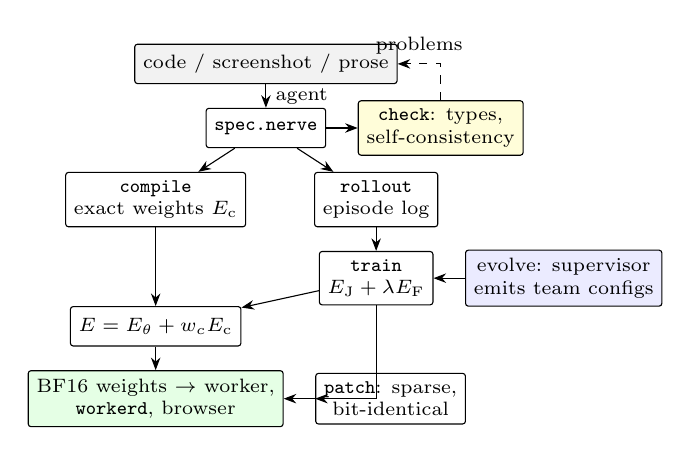
\begin{tikzpicture}[font=\scriptsize,node distance=3mm and 4mm,
  box/.style={draw,rounded corners=1pt,inner sep=3pt,minimum height=5mm,align=center},
  >={Stealth[length=1.6mm]}]
\node[box,fill=gray!10] (src) {code / screenshot / prose};
\node[box,below=of src] (spec) {\texttt{spec.nerve}};
\node[box,right=of spec,fill=yellow!15] (check) {\texttt{check}: types,\\ self-consistency};
\node[box,below=of spec,xshift=-14mm] (comp) {\texttt{compile}\\ exact weights $\Ec$};
\node[box,below=of spec,xshift=14mm] (roll) {\texttt{rollout}\\ episode log};
\node[box,below=of roll] (train) {\texttt{train}\\ $\Ej+\lambda\Ef$};
\node[box,below=of comp,yshift=-7mm] (energy) {$E=\Eth+w_c\Ec$};
\node[box,below=of energy,fill=green!10] (edge) {BF16 weights $\to$ worker,\\ \texttt{workerd}, browser};
\node[box,right=of train,fill=blue!8] (evo) {evolve: supervisor\\ emits team configs};
\node[box,right=of edge] (patch) {\texttt{patch}: sparse,\\ bit-identical};
\draw[->] (src) -- node[right]{agent} (spec);
\draw[->] (spec) -- (check);
\draw[->,dashed] (check.north) |- node[above,pos=0.75]{problems} (src.east);
\draw[->] (spec) -- (comp);
\draw[->] (spec) -- (roll);
\draw[->] (roll) -- (train);
\draw[->] (comp) -- (energy);
\draw[->] (train) -- (energy);
\draw[->] (energy) -- (edge);
\draw[->] (evo) -- (train);
\draw[->] (train.south) |- (patch);
\draw[->] (patch) -- (edge);
\end{tikzpicture}
\end{minipage}
\caption{Left: the counter spec. Right: the pipeline. The spec is the only source of truth; the oracle, the circuit, the training data and the evaluation are all derived from it.}
\label{fig:pipeline}
\end{figure}

A spec (\cref{fig:pipeline}, left) declares typed \emph{fields} $f_1,\dots,f_n$ with domains $D_1,\dots,D_n$ (bools, enums, bounded ints, floats with or without a step grid), \emph{actions} with typed parameters, a guarded pure \emph{transition} per action, \emph{invariants} over states, \emph{ensures} clauses over (old state, new state, parameters), \emph{futures}, and \emph{learn} holes.

\begin{definition}[Finite spec]
A spec is \emph{finite} when every field domain is finite (a float with a step grid counts) and no action has a continuous parameter. Its state space is $\Sset=\prod_i D_i$ and its action set $\Aset$ is the set of concrete action instances, one per combination of discrete parameter values. The transition function $T:\Sset\times\Aset\to\Sset$ applies the action's update expressions when its guard holds and is the identity otherwise. For a hole action, $T$ is the hole's \emph{fallback}.
\end{definition}

Expressions are evaluated by a whitelisted AST walker (arithmetic, comparisons, boolean operators, conditionals, \texttt{old.}$f$, and a fixed set of builtins); nothing is \texttt{eval}'d. The \emph{oracle} is the interpreter of $T$ together with a checker that returns, for a step $(s,a,s')$, the list of properties it breaks: a field out of type, an invariant false at $s'$, or an ensures clause false. The oracle is the only ``software'' in the traditional sense, and it is derived mechanically from the spec, never written per interface.

\paragraph{Self-check.} Before anything is trained, \texttt{nerve check} runs the spec against itself: for every $s\in\Sset$ satisfying the invariants and every $a\in\Aset$ it asserts that $T(s,a)$ satisfies the invariants and the ensures clauses (for non-finite specs, over 2{,}000 random samples). A spec whose own transitions break its own properties never reaches training. The check caught a real error while we were writing the slider spec (an ensures clause that was false whenever the guard failed), and it is the loop condition for agent intake.

\paragraph{Futures and holes.} Declarative dragging~\citep{dragology} describes a drag by the set of model states it may lead to (\texttt{closest}, \texttt{between}, \texttt{vary}). A \texttt{futures} block declares this set per gesture, and energy-based inference is literally scoring those candidates and taking the minimum. The full state space is the conservative default and is what we evaluate against. A \texttt{learn} hole, after ink's learnable holes with an \texttt{ensures \dots{} else} fallback~\citep{inklang}, names behavior the spec can only show: an action, a safe fallback transition, and examples. The oracle knows only the fallback; the examples are ground truth the spec cannot express, and they enter training as positives (oversampled $20\times$) while the compiled circuit is made silent on that action.

\paragraph{Intake.} Code, prose, or a screenshot is turned into a spec by an agent (Claude Code, or DeepSeek Harness) given the grammar and one of three prompts; the harness runs \texttt{nerve check} and sends back problems for up to three rounds. Three of the eight specs in this paper came from screenshots this way (\cref{sec:results}).

\section{Compiling the explicit part into weights}
\label{sec:compile}

Let $\bx(s)=[\onehot(s_1);\dots;\onehot(s_n);\psi(s)]\in\R^{d_s}$ be the state features, where $\psi$ collects the ordinal features of \cref{sec:energy} (the circuit ignores them), and let $\be_a\in\R^{|\Aset|}$ be the action one-hot. For a finite spec with $H=|\Sset|\,|\Aset|$ we build a two-layer ReLU network with one hidden unit per pair $k=(s_k,a_k)$:
\begin{equation}
\label{eq:circuit}
h_k(s,a)=\relu\!\big(\langle \bx(s),\mathbf{w}^s_k\rangle+\langle \be_a,\mathbf{w}^a_k\rangle-n\big),\qquad
\mathbf{y}(s,a)=\textstyle\sum_k h_k(s,a)\,\mathbf{w}^o_k,
\end{equation}
with $\mathbf{w}^s_k$ the one-hot block of $\bx(s_k)$, $\mathbf{w}^a_k=\be_{a_k}$, and $\mathbf{w}^o_k$ the one-hot block of $\bx(T(s_k,a_k))$, or $\mathbf{0}$ when $a_k$ is a hole action. The circuit's energy of a candidate successor is
\begin{equation}
\label{eq:circuit-energy}
\Ec(s,a,s')=1-\tfrac{1}{n}\,\langle \bx(s'),\mathbf{y}(s,a)\rangle .
\end{equation}

\begin{theorem}[The compiled energy is a Hamming distance]
\label{thm:circuit}
For every finite spec, every $s\in\Sset$, every non-hole $a\in\Aset$ and every $s'\in\Sset$,
$\Ec(s,a,s')=\dH\big(s',T(s,a)\big)/n$, where $\dH$ counts the fields on which two states differ. In particular $\Ec$ is $0$ exactly at the true successor and at least $1/n$ everywhere else. For a hole action, $\Ec(s,a,\cdot)\equiv 1$.
\end{theorem}
\begin{proof}
Fix $(s,a)$. The pre-activation of unit $k$ is $\sum_i \ind{s_i=s_{k,i}}+\ind{a=a_k}-n$. If $s=s_k$ and $a=a_k$ it equals $1$. If $s\neq s_k$, at least one field differs, so the sum is at most $(n-1)+1-n=0$; if $s=s_k$ but $a\neq a_k$ it is $n+0-n=0$. Hence exactly one unit fires, with value $1$, and $\mathbf{y}(s,a)=\mathbf{w}^o_{(s,a)}$, the one-hot block of $T(s,a)$. Then $\langle\bx(s'),\mathbf{y}\rangle=\sum_i\ind{s'_i=T(s,a)_i}=n-\dH(s',T(s,a))$, which gives the claim. For a hole action $\mathbf{w}^o=\mathbf{0}$, so $\langle\bx(s'),\mathbf{y}\rangle=0$ and $\Ec\equiv1$.
\end{proof}

\begin{corollary}[When the circuit decides]
\label{cor:dominate}
Let $E=\Eth+w_c\Ec$ for any learned term $\Eth$. If for a given $(s,a)$ the learned term satisfies $\Eth(s,a,T(s,a))-\min_{s'}\Eth(s,a,s')<w_c/n$, then $\arg\min_{s'}E(s,a,s')=T(s,a)$. In particular, whenever the learned term's spread $\max_{s'}\Eth-\min_{s'}\Eth$ is below $w_c/n$, the circuit decides every non-hole transition regardless of what was learned; on hole actions the circuit contributes a constant and the learned term decides.
\end{corollary}

\begin{remark}
The circuit is a lookup table in weight form: $H=|\Sset||\Aset|$ hidden units and $H(2d_s+|\Aset|)$ computed parameters (\counterH{} units and \counterCparams{} parameters for the counter, \negH{} and \negCparams{} for negotiation). Its value is not compression but that it lives in the same function space as the learned energy, sums with it, and is exact there. We compile only when $H\le 2\times10^5$; larger interfaces are carried by the learned model alone. The weight matters. With a fixed $w_c=1000$ and $n\le5$ the bound is $w_c/n\ge200$, and on the trained negotiation network the learned term's spread over candidates reaches \negspread{}: the circuit was being outvoted in principle and agreed with the learned term only because the learned term was right. We therefore set the weight \emph{per query}, $w_c=\max(1000,\,n\cdot\mathrm{spread}+1)$, in the Python runtime and in the Worker alike, which makes \cref{cor:dominate} unconditional; a test trains nothing, multiplies the learned weights by $50$, and checks that every compiled transition of every finite spec still matches the oracle while hole actions are still left to the learned term.
\end{remark}

\section{The learned energy}
\label{sec:energy}

\paragraph{Features.} Finite fields are one-hot. An \emph{ordinal} field (an int or gridded float with more than two values) additionally contributes $\psi(u)=[u,\sin 2\pi k u,\cos 2\pi k u]_{k=1..4}$ of its normalized value $u\in[0,1]$, so that ``same value'' and ``$+1$'' are compositional in feature space. Continuous fields contribute $\psi(u)$ only, differentiably. Actions are one-hot over instances; a continuous parameter enters through a linear map added to the action embedding.

\paragraph{JEPA term.} An encoder $f_\theta:\R^{d_s}\to\R^d$ ($d=64$; three-layer GELU MLPs throughout), an action embedding $\be_a\mapsto\bz_a\in\R^d$, and a predictor $g_\theta$ give
\begin{equation}
\hat\bz'=g_\theta\big(f_\theta(\bx(s)),\bz_a\big),\qquad \Ej(s,a,s')=\big\|\hat\bz'-\bar f(\bx(s'))\big\|_2^2 ,
\end{equation}
where $\bar f$ is an exponential moving average of $f_\theta$ (momentum $0.99$) with no gradient, as in BYOL and I-JEPA~\citep{grill2020byol,assran2023ijepa}. The network never reconstructs pixels or DOM; it predicts in representation space, which is the right level for \emph{what the interface does} as opposed to what it looks like. Rendering is a separate decoder and out of scope here.

\paragraph{Factored term.} For each discrete field $f$ with domain size $n_f$ and current index $i_f$, let $\bx_{-f}$ be the state features with $f$'s own one-hot and ordinal features masked to zero. Two small MLPs $H_f,G_f$ read $[\bz_a;\bx_{-f}]$ and produce absolute logits $H_f\in\R^{n_f}$ and, for ordinal fields, shift logits $G_f\in\R^{2n_f-1}$ indexed by offset. The logit of next value $j$ is
\begin{equation}
\label{eq:factored}
\ell_f(j\mid s,a)=H_f(\bz_a,\bx_{-f})[j]+\ind{f\text{ ordinal}}\,G_f(\bz_a,\bx_{-f})[\,j-i_f+n_f-1\,]+\epsilon\,O_f(\hat\bz')[j],
\end{equation}
with $\epsilon=0.1$ a small own-value term for genuine exceptions, and $\Ef(s,a,s')=-\sum_f\log\operatorname{softmax}(\ell_f)[s'_f]$.

\begin{proposition}[Shift equivariance along ordinal fields]
\label{prop:equiv}
Fix $a$ and all fields other than $f$. Write $\ell^{\mathrm{shift}}_i(j)=G_f(\bz_a,\bx_{-f})[j-i+n_f-1]$ for the shift contribution when the current value has index $i$. Then $\ell^{\mathrm{shift}}_{i+\delta}(j+\delta)=\ell^{\mathrm{shift}}_i(j)$ for all $i,j,\delta$ with both indices in range, and $H_f(\bz_a,\bx_{-f})$ does not depend on $i$ at all.
\end{proposition}
\begin{proof}
$G_f$ and $H_f$ receive $\bx_{-f}$, which by construction carries no information about $f$'s value, so they are constant in $i$; the shift index $j-i$ is invariant under $(i,j)\mapsto(i+\delta,j+\delta)$.
\end{proof}

So a rule such as \texttt{count: "min(count + 1, 9)"} under guard \texttt{armed}, once learned at $i=3$, is the same function at $i=8$; what the head \emph{can} condition on is the action and every other field, which is exactly what guards refer to. Only the $\epsilon$-weighted own-value term and the domain boundary break the symmetry, and the boundary is where the examples differ anyway (\texttt{min}, \texttt{max}, \texttt{clamp}). \Cref{sec:results} shows where this matters: on the specs whose rules are shifts, increasingly as more cells are held out, and not at all on the negotiation game.

\paragraph{Total energy and inference.} $E=\Ej+\lambda_F\Ef+w_c\Ec$ with $\lambda_F=10$ and $w_c$ set per query as in \cref{sec:compile}. For finite specs inference is $\arg\min$ over all states (or the declared futures). For a spec with continuous fields, candidates are the discrete combinations times a handful of seeds per continuous field (the current value, the action's parameter, $0$, $\tfrac12$, $1$, and six random points); each seed is descended on $\Ej$ with Adam ($60$ steps, step size $0.05$, clamped to the range) and the global minimum wins---dragging's \texttt{vary} as gradient descent on an energy.

\paragraph{Training.} A run is a pure function of (spec, log, config, seed). The log is an append-only JSONL file written by policies that operate the oracle: \emph{exhaustive} (every (state, action) pair once, for finite specs under $2\times10^5$ pairs), \emph{coverage}, \emph{random}, and \emph{adversary} (prefers boundary-hugging actions). Every positive comes with $k=3$ spec-derived negatives: candidate successors that break an invariant or an ensures clause, or are plainly wrong. The loss on a batch is
\begin{equation}
\begin{aligned}
\mathcal{L}={}&\underbrace{\mathrm{CE}\big(-\Ej(s,a,\cdot)/\tau,\ T(s,a)\big)}_{\text{InfoNCE over all candidates}}
+0.1\,\Ej(s,a,T(s,a))
+\underbrace{\big[m+\bar E_{+}-\Ej(s,a,s'_{-})\big]_+}_{\text{hinge on violating futures}}\\
&+0.05\,\mathcal{L}_{\mathrm{var}}+\mathcal{L}_{\mathrm{ord}}+\lambda_F\,\Ef(s,a,T(s,a)),
\end{aligned}
\end{equation}
with $\tau=0.1$, margin $m=1$, $\mathcal{L}_{\mathrm{var}}$ the VICReg variance hinge~\citep{bardes2022vicreg} (skipped on a batch of one, which otherwise produces a NaN that silently zeroes a run), and $\mathcal{L}_{\mathrm{ord}}$ a linear read-out of ordinal values from both $f_\theta(\bx(s))$ and $\hat\bz'$. AdamW with weight decay $0.05$---the grokking lever~\citep{power2022grokking,nanda2023progress}---learning rate $3\times10^{-3}$ with cosine decay, batch $128$, $300$ epochs. Held-out cells (\cref{sec:protocol}) are excluded from positives and negatives alike.

\section{Measuring a network as a program}
\label{sec:protocol}

A program is right or wrong on every input, so we report exact match, not likelihood. Let $P$ be the set of (valid state, non-hole action) pairs. A salted BLAKE2b hash of the pair assigns $15\%$ of $P$ to a \emph{held-out} set, so the split is a property of the spec and the salt, not of the run; training never sees those cells, and tiny specs with fewer than $20$ pairs get no hold-out at all (toggle). We report:
\emph{held-out exact}, the fraction of held-out cells where $\arg\min E$ equals $T$;
\emph{all exact}, the same over $P$;
\emph{violation rate}, the fraction of predicted successors over $P$ that break an invariant or ensures clause---a wrong but legal answer is a bug, an illegal one is a safety failure;
\emph{learned-only exact}, all-exact with the circuit disabled, so the network cannot hide behind the compiler;
and \emph{hole accuracy} on the examples of each \texttt{learn} hole. The official score is $0.4\,\text{held-out}+0.2\,\text{all}+0.2\,(1-\text{violations})+0.2\,\text{learned-only}$, blended $80/20$ with hole accuracy when the spec has holes; it is the single number the evolving team optimizes. Two rules matter more than the weights: every number is computed from the BF16 checkpoint that ships, never from the FP32 training copy, and the Worker that serves the network must agree with Python on every transition over HTTP before a number is reported. Training and evaluation share one hold-out function; an earlier version in which they disagreed for tiny specs reported held-out cells as seen, and we count that bug, with the NaN above, as having mattered more than any modelling idea.

\section{Results}
\label{sec:results}

\paragraph{Specs.} Five hand-written specs (toggle; the counter of \cref{fig:pipeline} with a \texttt{learn} hole; a gridded slider; the same slider with a continuous \texttt{value} and \texttt{to}; and a finite Deal-or-No-Deal in which two agents split two books and two hats over at most three rounds, $216$ states $\times$ $11$ action instances) and three specs produced from screenshots of real controls by the intake agent (a push-notifications toggle with a draggable knob, $84\times27$; a guest-count stepper, $8\times3$; a volume slider with mute, $404\times103$). The screenshot specs went image $\to$ spec (one or two rounds of \texttt{nerve check} feedback) $\to$ exhaustive log $\to$ network with no hand edits.

\begin{table}[t]
\centering
\caption{Learned-only conformance (compiled circuit disabled; $15\%$ of (state, action) cells held out of training). \textbf{Top:} runs from the repository record, one Hugging Face \texttt{a10g-small} job each, $300$ epochs. \textbf{Bottom:} the four hand-written finite specs re-run for this paper on a two-core CPU with the same configuration and three seeds; we give the held-out count and the per-seed values. Toggle has two cells and no hold-out set.}
\label{tab:main}
\footnotesize
\setlength{\tabcolsep}{4pt}
\begin{tabular}{llrrccc}
\toprule
spec & source & $|\Sset|\times|\Aset|$ & held-out & held-out exact & all exact & viol.\\
\midrule
\multicolumn{7}{l}{\emph{repository record (GPU, one seed)}}\\
toggle & hand & $2\times1$ & -- & 1.000 & 1.000 & 0\\
counter (with hole) & hand & $20\times14$ & 34 & 1.000 & 1.000 & 0\\
slider (gridded) & hand & $50\times29$ & 213 & 1.000 & 1.000 & 0\\
negotiate & hand & $216\times11$ & 367 & 1.000 & 1.000 & 0\\
push-notifications toggle & screenshot & $84\times27$ & & 1.000 & 1.000 & 0\\
guest stepper & screenshot & $8\times3$ & & 1.000 & 1.000 & 0\\
volume slider & screenshot & $404\times103$ & & 1.000 & 1.000 & 0\\
slider (continuous) & hand & $2\times\infty$ & 1{,}000 & \multicolumn{2}{c}{0.998 within 1\% of range} & 0.002\\
\midrule
\multicolumn{7}{l}{\emph{re-run for this paper (CPU, seeds 0/1/2)}}\\
toggle & hand & $2\times1$ & -- & 1.000/1.000/1.000 & 1.000/1.000/1.000 & 0/0/0\\
counter (with hole) & hand & $20\times14$ & 34 & 0.971/0.971/1.000 & 0.996/0.996/1.000 & 0/0/0\\
slider (gridded) & hand & $50\times29$ & 213 & 1.000/1.000/0.995 & 1.000/1.000/0.999 & 0/0/0\\
negotiate & hand & $216\times11$ & 367 & 1.000/1.000/1.000 & 1.000/1.000/1.000 & 0/0/0\\
\bottomrule

\end{tabular}
\end{table}

\paragraph{Conformance.} \Cref{tab:main} gives the repository's numbers and our re-runs. \mainsummary{} With the circuit enabled, all-exact is $1.000$ on every finite spec by \cref{thm:circuit}, and the hole examples of the counter are learned (\holesummary{}). The continuous slider, evaluated at $1{,}000$ random (state, action) pairs with inference by gradient descent, reaches $0.998$ within $1\%$ of the range in the repository's GPU run; our CPU re-run with the same training configuration ($200$ epochs, $d=128$) but the default $40$-episode log reaches only \contexactcpu{}, with $8\%$ of predictions breaking the spec's clamp or guard, and since that row's episode log was not committed we cannot say whether data or hardware accounts for the gap. (The gridded slider had reached $0.986$ before the factored head and ordinal features were added.)

\begin{table}[t]
\centering
\caption{Ablations on the three hand-written specs with ordinal fields (learned-only, $15\%$ held out, seed 0 unless noted): held-out exact match and cells. At this hold-out the JEPA term alone is nearly sufficient; the factored head recovers the last cells on the two shift-rule specs and is irrelevant on negotiation.}
\label{tab:ablate}
\footnotesize
\setlength{\tabcolsep}{4pt}
\begin{tabular}{lccc}
\toprule
 & negotiate & slider & counter\\
\midrule
full model (JEPA + ordinal read-out + factored head) & 1.000 (367/367) & 1.000 (213/213) & 0.971 (33/34)\\
\quad without factored head & 1.000 (367/367) & 0.991 (211/213) & 0.941 (32/34)\\
\quad without factored head and ordinal read-out & 1.000 (367/367) & 0.991 (211/213) & 0.971 (33/34)\\
\quad weight decay $10^{-4}$ (default $0.05$) & 1.000 (367/367) & 1.000 (213/213) & 0.971 (33/34)\\
\quad without factored head, seeds 0--2 & 1.000/1.000/1.000 & & \\
\bottomrule

\end{tabular}
\end{table}

\paragraph{What does the work.} \Cref{tab:ablate} removes the pieces one at a time at the standard $15\%$ hold-out, and \cref{fig:holdout} holds out $30\%$ and $50\%$ of the cells. Three things are visible. First, with exhaustive logs, ordinal features and weight decay in place, the JEPA term alone is already close: negotiation is exact on every held-out cell without the factored head, without the ordinal read-out, and with weight decay $10^{-4}$, and it stays exact when half of its $2{,}376$ cells are held out---the rules of the game (\texttt{propose} assigns the parameters, flips the turn and increments the round; \texttt{accept} and \texttt{walk} set the status under a guard) are recovered from the other half. Second, where a rule is a shift along an ordinal field the factored head is what carries the held-out cells, and increasingly so as fewer cells are seen: the slider goes from $211$ to $213$ of $213$ at $15\%$ and from $436$ to $448$ of $449$ at $30\%$; the counter from $32$ to $33$ of $34$ and from $67$ to $71$ of $76$. Third, the counter is the hard case: $20$ states, a guard (\texttt{armed}) that silences two actions, a hole, and range boundaries two cells from the middle; at $50\%$ hold-out it reaches $122$ of $131$ with one predicted successor breaking an ensures clause, the only violation in the sweep. \Cref{fig:curves} shows that generalization is not slow: every spec is exact on its held-out cells by epoch $20$; the counter's single miss on seed~$0$ appears at epoch $110$, after a hundred epochs of being right, which argues for a validation split separate from the held-out test cells rather than for more training.

\begin{figure}[t]
\centering
\begin{subfigure}[t]{0.48\textwidth}
\centering
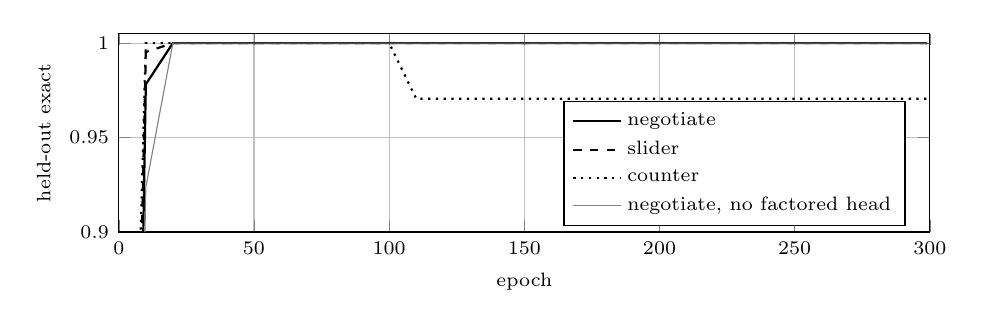
\begin{tikzpicture}
\begin{axis}[width=0.98\linewidth,height=4.1cm,xlabel={epoch},ylabel={held-out exact},ymin=0.9,ymax=1.005,xmin=0,xmax=300,
legend style={at={(0.97,0.03)},anchor=south east,font=\scriptsize,cells={anchor=west}},grid=major,font=\scriptsize]
\addplot[thick] coordinates {(0,0.1471) (10,0.9782) (20,1.0000) (30,1.0000) (40,1.0000) (50,1.0000) (60,1.0000) (70,1.0000) (80,1.0000) (90,1.0000) (100,1.0000) (110,1.0000) (120,1.0000) (130,1.0000) (140,1.0000) (150,1.0000) (160,1.0000) (170,1.0000) (180,1.0000) (190,1.0000) (200,1.0000) (210,1.0000) (220,1.0000) (230,1.0000) (240,1.0000) (250,1.0000) (260,1.0000) (270,1.0000) (280,1.0000) (290,1.0000) (299,1.0000)}; \addlegendentry{negotiate}
\addplot[thick,dashed] coordinates {(0,0.3333) (10,0.9953) (20,1.0000) (30,1.0000) (40,1.0000) (50,1.0000) (60,1.0000) (70,1.0000) (80,1.0000) (90,1.0000) (100,1.0000) (110,1.0000) (120,1.0000) (130,1.0000) (140,1.0000) (150,1.0000) (160,1.0000) (170,1.0000) (180,1.0000) (190,1.0000) (200,1.0000) (210,1.0000) (220,1.0000) (230,1.0000) (240,1.0000) (250,1.0000) (260,1.0000) (270,1.0000) (280,1.0000) (290,1.0000) (299,1.0000)}; \addlegendentry{slider}
\addplot[thick,dotted] coordinates {(0,0.4706) (10,1.0000) (20,1.0000) (30,1.0000) (40,1.0000) (50,1.0000) (60,1.0000) (70,1.0000) (80,1.0000) (90,1.0000) (100,1.0000) (110,0.9706) (120,0.9706) (130,0.9706) (140,0.9706) (150,0.9706) (160,0.9706) (170,0.9706) (180,0.9706) (190,0.9706) (200,0.9706) (210,0.9706) (220,0.9706) (230,0.9706) (240,0.9706) (250,0.9706) (260,0.9706) (270,0.9706) (280,0.9706) (290,0.9706) (299,0.9706)}; \addlegendentry{counter}
\addplot[gray] coordinates {(0,0.1717) (10,0.9237) (20,1.0000) (30,1.0000) (40,1.0000) (50,1.0000) (60,1.0000) (70,1.0000) (80,1.0000) (90,1.0000) (100,1.0000) (110,1.0000) (120,1.0000) (130,1.0000) (140,1.0000) (150,1.0000) (160,1.0000) (170,1.0000) (180,1.0000) (190,1.0000) (200,1.0000) (210,1.0000) (220,1.0000) (230,1.0000) (240,1.0000) (250,1.0000) (260,1.0000) (270,1.0000) (280,1.0000) (290,1.0000) (299,1.0000)}; \addlegendentry{negotiate, no factored head}
\end{axis}
\end{tikzpicture}

\caption{Held-out exact match during training (axis starts at $0.9$); all three specs are exact by epoch $20$.}
\label{fig:curves}
\end{subfigure}\hfill
\begin{subfigure}[t]{0.48\textwidth}
\centering
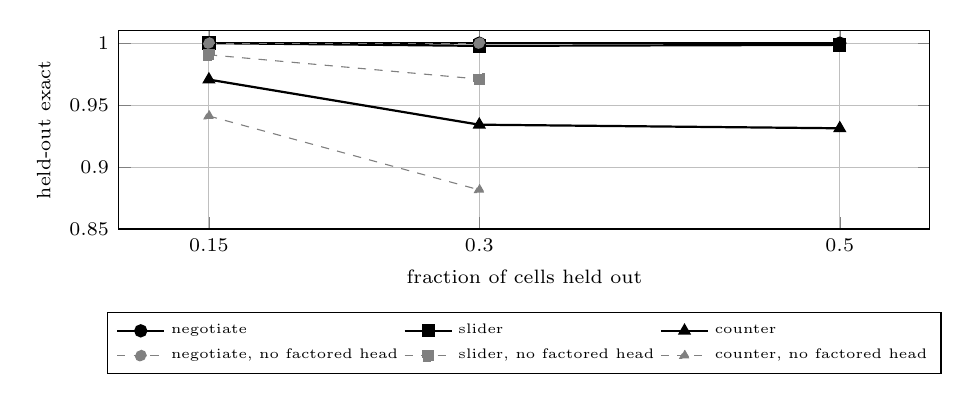
\begin{tikzpicture}
\begin{axis}[width=0.98\linewidth,height=4.1cm,xlabel={fraction of cells held out},ylabel={held-out exact},
ymin=0.85,ymax=1.01,xmin=0.1,xmax=0.55,xtick={0.15,0.3,0.5},legend style={at={(0.5,-0.42)},anchor=north,font=\tiny,cells={anchor=west}},legend columns=3,grid=major,font=\scriptsize]
\addplot[mark=*,thick] coordinates {(0.15,1.0000) (0.3,1.0000) (0.5,1.0000)}; \addlegendentry{negotiate}
\addplot[mark=square*,thick] coordinates {(0.15,1.0000) (0.3,0.9978) (0.5,0.9986)}; \addlegendentry{slider}
\addplot[mark=triangle*,thick] coordinates {(0.15,0.9706) (0.3,0.9342) (0.5,0.9313)}; \addlegendentry{counter}
\addplot[mark=*,dashed,gray] coordinates {(0.15,1.0000) (0.3,1.0000)}; \addlegendentry{negotiate, no factored head}
\addplot[mark=square*,dashed,gray] coordinates {(0.15,0.9906) (0.3,0.9710)}; \addlegendentry{slider, no factored head}
\addplot[mark=triangle*,dashed,gray] coordinates {(0.15,0.9412) (0.3,0.8816)}; \addlegendentry{counter, no factored head}
\end{axis}
\end{tikzpicture}

\caption{Held-out exact match as the held-out fraction grows (learned-only, seed 0).}
\label{fig:holdout}
\end{subfigure}
\caption{Generalization inside an interface (learned-only, seed 0). Negotiation is recovered from half of its cells with or without the factored head; the shift-rule specs need it as more is held out; the counter loses one held-out cell late in training.}
\label{fig:gen}
\end{figure}

\paragraph{Margins.} On the negotiation network the energy gap between the true successor and the runner-up, learned-only, is at least \negmarginmin{} on held-out cells (median \negmarginmed{}) and at least \negmarginminseen{} on seen cells: held-out cells are not decided by a hair. The gap is in units dominated by $\lambda_F\Ef$, i.e.\ roughly $10\times$ a log-probability ratio.

\paragraph{Cost.} Every network here has between $10^5$ and $2\times10^5$ learned parameters and trains in $34$ s to $9$ min on an \texttt{a10g-small}, or \negcpu{} min for negotiation on two CPU cores. Inference is one forward pass plus the target encodings of the $|\Sset|$ candidates (cached in the Worker); a step on the $216$-candidate negotiation network takes about $1.4$~ms in Python on one CPU core and $0.6$~ms on the counter.

\section{Shipping it}
\label{sec:ship}

\paragraph{BF16 and the edge.} The checkpoint is BF16. \texttt{nerve export} writes the weights, the compiled circuit, the state vectors and the feature layout to one JSON document; \texttt{edge/src/nn.ts} (under 200 lines) is the entire runtime: GELU MLPs, the factored head, the circuit, and an argmin. The same bundle runs as a Cloudflare Worker with Durable Object sessions and R2 weights, locally on \texttt{workerd} with disk-backed weights, and as a static page in which the network runs in the browser (\texttt{docs/play}, all seven finite networks). The test suite trains small models, starts \texttt{workerd} on a spare port, and asserts that Python and the Worker agree on the state of every transition and on its energy to within $0.05$ over HTTP; the weights agree bit for bit by digest, the energies only to tolerance because the Worker's GELU is the tanh approximation and PyTorch's is exact.

\paragraph{Sparse patches.} Continued training at the learning rates used for RL post-training changes few BF16 bits; \citet{miahi2026pulse} measure $\sim$$99\%$ update sparsity on 0.5--7B models and propose PULSE: send only changed indices and their new absolute values, verify a digest. We implement the same format (varint index deltas, BF16 values, zstd, SHA-256 of the full post-patch checkpoint) in Python and in the Worker; a patch is applied as a memory copy and rejected---weights restored---if the digest does not match, and a corrupted frame is likewise refused. On the negotiation network ($140$k parameters) one further epoch at $3\times10^{-6}$ changes \pulseonesparsity{} of BF16 values and ships as a \pulseonekb{}~kB patch against a $280$~kB checkpoint; \pulsesummary{} Our networks are three to five orders of magnitude smaller than the models PULSE was designed for, so the ratios are smaller too; the property we rely on is bit-identity, not compression.

\paragraph{An evolving team built the last one.} \citet{cao2026eat} describe an Evolving Agent Team: a supervisor agent that never writes the solution and each iteration reflects on the last team's result and emits a team configuration (roles, prompts, phases, ownership); the team, made of coding agents, does the work; a fixed evaluation scores it. \texttt{nerve evolve} is that loop over this pipeline: roles own \texttt{spec}, \texttt{rollout}, \texttt{adversary}, \texttt{train} or \texttt{eval}; a spec role may add missing guards and properties to a working copy but every edit must pass \texttt{nerve check} or is reverted; only the harness trains. An offline rule-based reflector makes the loop reproducible with no model at all (and is what the tests run). With Claude Code as supervisor and role agents, and one GPU job per iteration, the negotiation spec ran $11$ iterations for \$14.23, reached $1.0$ on every metric, invented four roles that did not exist at iteration~0 (\texttt{split\_prober}, \texttt{spec\_verifier}, \texttt{margin\_auditor}, \texttt{margin\_checker}), and, once the score was saturated, restructured the team to cut its own cost per iteration. The run's record (every team configuration, evaluation and role report) is part of the artifact; see \cref{sec:limits} on its provenance.

\section{Related work}
\label{sec:related}

\paragraph{Programs in weights.} That finite automata can be constructed in networks is classical~\citep{omlin1996constructing,siegelmann1995computational}; Tracr compiles RASP programs into transformer weights~\citep{lindner2023tracr}, Cajal compiles a typed linear language to linear and recurrent neurons with a correctness proof~\citep{cajal,cajalrec}, ink's \texttt{emit-circuit} lowers functions over finite types to exact ReLU nets~\citep{inklang}, and Qwenputer and qwenGPU compile a CPU and a GPU into layers in front of a pretrained language model~\citep{qwenputer,qwengpu}. Our circuit is the simplest member of this family---a table---and its contribution is the energy framing (\cref{thm:circuit}) that lets it sum with a learned term and be silent where the spec is.

\paragraph{Energy-based inference and JEPA.} Scoring candidates and taking the minimum is energy-based learning~\citep{lecun2006tutorial}; implicit behavioral cloning trains energy policies with InfoNCE over sampled actions and infers by argmin or descent~\citep{florence2021ibc}. JEPA predicts in representation space with an EMA target~\citep{lecun2022path,assran2023ijepa,grill2020byol}; latent world models plan by descending prediction error~\citep{zhou2024dinowm,sobal2025pldm}. We use the prediction error as the energy of a program and add a factored equivariant term because, for a state machine, the field-wise structure is known.

\paragraph{Neural interfaces and games.} NeuralOS~\citep{rivard2026neuralos}, GameNGen~\citep{valevski2024gamengen} and Genie~\citep{bruce2024genie} learn interactive systems as frame predictors from recordings. They answer what the screen will look like; we answer what the state will be, hold the answer to a spec, and treat rendering as a separate decoder. The end-to-end negotiator~\citep{lewis2017deal} learned a dialogue policy; our negotiation spec is a referee for such policies.

\paragraph{Specifications and holes.} Typed holes with live semantics~\citep{omar2019hazel}, program sketching~\citep{solar2008sketch} and neurosymbolic programs with neural holes~\citep{gaunt2016terpret,chaudhuri2021neurosymbolic} are the ancestors of \texttt{learn}; declarative dragging~\citep{dragology} is the ancestor of \texttt{futures}; TLA$^+$ and Alloy~\citep{lamport2002tla,jackson2012alloy} are the ancestors of the self-check. Weight update sparsity and PULSE are from \citet{miahi2026pulse}; the evolving-team loop is from \citet{cao2026eat}; grokking with weight decay from \citet{power2022grokking,nanda2023progress}.

\section{Limitations, and what this is not}
\label{sec:limits}

\emph{The interfaces are small.} The largest finite spec has $404$ states and $103$ action instances; the circuit is a table, and ``learned-only $1.0$'' on $41{,}612$ cells is generalization \emph{within} one interface from $85\%$ of its cells to the rest, not generalization across interfaces. Nothing here transfers from one spec to another; a shared backbone is future work.
\emph{The oracle is code.} The spec is executed by an interpreter derived from it; ``software without code'' means the shipped artifact is weights, not that no program exists. The interpreter is small, generic, and never written per interface, which is the point.
\emph{The circuit's guarantee was conditional until this paper.} \Cref{cor:dominate} needs the learned term's spread below $w_c/n$ and the trained networks exceeded it; the per-query weight of \cref{sec:compile} was added while writing, and the runs in \cref{tab:main,tab:ablate} predate it (they are learned-only and unaffected).
\emph{Rendering is out of scope.} The network is the behavior; what the interface looks like is a decoder we do not learn.
\emph{Seeds and splits.} Our re-runs use three seeds and one hash salt; the held-out \emph{set} is fixed across seeds, so the seed variance we report covers initialization and shuffling, not split choice. Worse, the evolving team optimizes the official score, which is computed on those same held-out cells, so in an evolution run they are a validation set and the reported number is optimistic; the artifact now takes a salt so that a second, sealed split can be the test.
\emph{The evolution record.} The $11$-iteration run is recorded in the repository's working tree under \texttt{docs/runs/}, a path that the branch's \texttt{.gitignore} excluded at the time of writing; the record must be committed before the claim can be checked by a reader, and we treat it as a case study rather than a result until then.
\emph{Negotiation is finite and silent.} The game has no language; it is the rules of the game held in weights, which is the first half of the original repository's task and not the second.

\section{Conclusion}
\label{sec:conclusion}

A small interactive program can be shipped as a network and held to its specification: compiled where the spec is explicit, trained where it is not, scored on the weights that ship, and executed by one function at the edge. Exhaustive coverage of the seen cells mattered as much as any modelling idea; the idea that mattered where coverage was thin was an equivariant factored energy that makes a shift rule the same function at every value of a field; the two bugs that mattered were a NaN and a split disagreement. The next steps are in the repository's roadmap: factored and verified circuits, hard refusal at the edge, a shared backbone across specs, and bringing the 2017 dataset back so that two language agents negotiate over a state the network also enforces. One of them deserves a sentence here. Dragology's drag operators each return, per pointer frame, a preview state, a drop state and a \emph{gap}---the distance from the pointer to where the dragged element lands in that state---and \texttt{closest}, \texttt{between} and \texttt{vary} are argmin, convex relaxation and gradient descent on that gap~\citep{dragology}. The gap is an energy, so a drag is one minimization of $E_{\mathrm{spec}}+\lambda\,\mathrm{gap}$ over futures the spec derives rather than the author lists; the operator memory (stickiness, lock, far/near) is a small guarded state machine the spec language already has words for; and the shift kernel of \cref{sec:energy} is the ordinal case of a rule---equivariance chosen by the field's type---whose list case (permutation equivariance) is exactly what Dragology's reordering demos need. The design is written out in the repository (\texttt{docs/dragology.md}).

\paragraph{Reproducibility.} \texttt{scripts/demo.sh counter} runs the pipeline on a CPU in about a minute; the sweep script and raw results behind \cref{tab:main,tab:ablate,fig:gen} are in \texttt{docs/paper/} and regenerate every number in this paper.

\bibliographystyle{plainnat}
\bibliography{refs}

\appendix
\section{The spec language}
\label{app:grammar}

A \texttt{.nerve} file is YAML with the following keys. Types: \texttt{\{type: int, range: [lo, hi]\}}, \texttt{\{type: enum, values: [\dots]\}}, \texttt{\{type: bool\}}, \texttt{\{type: float, range: [lo, hi], step: s\}} (gridded) or without \texttt{step} (continuous).

\begin{lstlisting}
nerve: 1
name: <identifier>
state:        { <field>: <type>, ... }
actions:      { <action>: {} | {params: {<p>: <type>}}, ... }
transitions:  { <action>: { when: "<guard>", <field>: "<expr>", ... }, ... }
invariants:   [ "<expr over state>", ... ]
ensures:      [ { after: <action> | omitted, holds: "<expr over new state, params, old.*>" }, ... ]
futures:      { <gesture>: { kind: closest | between | vary, over: <field>, values: [...] } }
learn:        [ { name, action, fallback: {<field>: "<expr>"},
                  examples: [ { state: {...}, params: {...}, next: {...} } ] } ]
initial:      { <field>: <value> }
\end{lstlisting}

Expressions: literals, field names, parameter names, \texttt{old.}$f$, the operators \texttt{+ - * / // \% **}, chained comparisons, \texttt{and/or/not}, \texttt{x if c else y}, and the builtins \texttt{min max abs clamp len int bool}. The parser rejects any other syntax node, any call that is not a builtin, and any attribute access that is not on \texttt{old}. YAML's \texttt{on}/\texttt{off}/\texttt{yes}/\texttt{no} are strings, not booleans, so enum values such as \texttt{[off, on]} survive. A hole example must give every field of \texttt{state} and \texttt{next} and, if the hole's action takes parameters, a \texttt{params} block; an example outside the declared types is a parse error.

\paragraph{The negotiation spec.} Two agents split two books and two hats; a proposal is what the proposer keeps; at most three rounds; terminal states absorb.
\begin{lstlisting}
nerve: 1
name: negotiate
state:
  turn:   {type: enum, values: [a, b]}
  books:  {type: int, range: [0, 2]}
  hats:   {type: int, range: [0, 2]}
  status: {type: enum, values: [open, deal, no_deal]}
  rounds: {type: int, range: [0, 3]}
actions:
  propose: {params: {b: {type: int, range: [0, 2]}, h: {type: int, range: [0, 2]}}}
  accept: {}
  walk: {}
transitions:
  propose: { when: "status == 'open' and rounds < 3",
             books: "b", hats: "h", turn: "'b' if turn == 'a' else 'a'", rounds: "rounds + 1" }
  accept:  { when: "status == 'open' and rounds > 0", status: "'deal'" }
  walk:    { when: "status == 'open'", status: "'no_deal'" }
invariants: ["0 <= books <= 2 and 0 <= hats <= 2", "rounds <= 3"]
ensures:
  - { after: propose, holds: "turn != old.turn or old.status != 'open' or old.rounds >= 3" }
  - { after: accept,  holds: "status != 'open' or old.rounds == 0" }
  - { holds: "status == old.status or old.status == 'open'" }
initial: {turn: a, books: 0, hats: 0, status: open, rounds: 0}
\end{lstlisting}

\section{Encoding, sizes and hyper-parameters}
\label{app:details}

\begin{table}[h]
\centering
\caption{Per-spec sizes. $d_s$ is the state feature width (one-hots plus $9$ ordinal features per ordinal field), $|\Aset|$ the number of action instances, $H$ the number of compiled hidden units, and ``learned'' the number of trainable parameters of the JEPA and factored head ($d=64$, hidden $128$).}
\label{tab:sizes}
\small
\begin{tabular}{lrrrrrr}
\toprule
spec & $|\Sset|$ & $|\Aset|$ & $d_s$ & $H$ & circuit params & learned params\\
\midrule
toggle & 2 & 1 & 2 & 2 & 10 & \toggleparams\\
counter & 20 & 14 & 21 & 280 & 15{,}680 & \counterparams\\
slider (gridded) & 50 & 29 & 36 & 1{,}450 & 146{,}450 & \sliderparams\\
negotiate & 216 & 11 & 42 & 2{,}376 & 225{,}720 & \negparams\\
push-notifications toggle & 84 & 27 & 34 & 2{,}268 & -- & 126{,}594$^\dagger$\\
guest stepper & 8 & 3 & 17 & 24 & -- & 102{,}961$^\dagger$\\
volume slider & 404 & 103 & 114 & 41{,}612 & -- & 188{,}338$^\dagger$\\
\bottomrule
\end{tabular}

\smallskip
{\footnotesize $^\dagger$Counted from the exported browser weights (includes the factored head's mask buffer); the specs themselves were not yet committed at the time of writing.}
\end{table}

Training configuration for every finite run in this paper unless stated: $300$ epochs, batch $128$, AdamW ($\beta$ defaults) with learning rate $3\times10^{-3}$, cosine decay to $5\%$, weight decay $0.05$, EMA momentum $0.99$, InfoNCE temperature $\tau=0.1$, hinge margin $1$, variance weight $0.05$, ordinal read-out weight $1$, factored weight $\lambda_F=10$, own-value scale $\epsilon=0.1$, hole oversampling $20\times$, hold-out $15\%$, circuit weight $w_c=1000$. The continuous slider used $200$ epochs and $d=128$. The episode log for each spec is produced by \texttt{nerve rollout} with its default policies (exhaustive, coverage, random, adversary; $40$ episodes of horizon $20$ each; $3$ negatives per positive). Rollout knobs are capped ($400$ episodes, horizon $60$, $10$ negatives) because an agent once asked for $26{,}000$ negatives per step and produced a $2.5$~GB log.

\section{Every run}
\label{app:runs}

\Cref{tab:allruns} lists every training run behind \cref{tab:main,tab:ablate,fig:gen}, from the raw \texttt{results.jsonl} written by the sweep script. ``held'' is held-out exact match with the number of held-out cells, ``all'' is exact match over all valid cells, ``viol'' the violation rate, ``holes'' the hole-example accuracy where the spec has holes.

\begin{table}[h]
\centering
\caption{All CPU runs for this paper (learned-only unless the tag says \texttt{circuit}).}
\label{tab:allruns}
\scriptsize
\begin{tabular}{llrrrrrrr}
\toprule
tag & configuration & held & $n_{\text{held}}$ & all & viol & holes & params & wall (s)\\
\midrule
\texttt{toggle\_main\_s0} & s0 & 1.000 & 2 & 1.000 & 0 & -- & 96,196 & 32\\
\texttt{counter\_main\_s0} & s0 & 0.971 & 34 & 0.996 & 0 & 1.00 & 111,212 & 51\\
\texttt{slider\_main\_s0} & s0 & 1.000 & 213 & 1.000 & 0 & -- & 121,832 & 774\\
\texttt{negotiate\_main\_s0} & s0 & 1.000 & 367 & 1.000 & 0 & -- & 140,018 & 322\\
\texttt{toggle\_main\_s1} & s1 & 1.000 & 2 & 1.000 & 0 & -- & 96,196 & 32\\
\texttt{counter\_main\_s1} & s1 & 0.971 & 34 & 0.996 & 0 & 1.00 & 111,212 & 38\\
\texttt{slider\_main\_s1} & s1 & 1.000 & 213 & 1.000 & 0 & -- & 121,832 & 57\\
\texttt{negotiate\_main\_s1} & s1 & 1.000 & 367 & 1.000 & 0 & -- & 140,018 & 108\\
\texttt{toggle\_main\_s2} & s2 & 1.000 & 2 & 1.000 & 0 & -- & 96,196 & 35\\
\texttt{counter\_main\_s2} & s2 & 1.000 & 34 & 1.000 & 0 & 1.00 & 111,212 & 38\\
\texttt{slider\_main\_s2} & s2 & 0.995 & 213 & 0.999 & 0 & -- & 121,832 & 57\\
\texttt{negotiate\_main\_s2} & s2 & 1.000 & 367 & 1.000 & 0 & -- & 140,018 & 340\\
\texttt{negotiate\_nofact\_s0} & s0, no fact & 1.000 & 367 & 1.000 & 0 & -- & 102,723 & 1267\\
\texttt{slider\_nofact\_s0} & s0, no fact & 0.991 & 213 & 0.999 & 0 & -- & 102,209 & 45\\
\texttt{counter\_nofact\_s0} & s0, no fact & 0.941 & 34 & 0.992 & 0 & 1.00 & 97,409 & 31\\
\texttt{negotiate\_purejepa\_s0} & s0, no fact, no ord & 1.000 & 367 & 1.000 & 0 & -- & 102,723 & 62\\
\texttt{negotiate\_wd1e-4\_s0} & s0, wd 0.0001 & 1.000 & 367 & 1.000 & 0 & -- & 140,018 & 103\\
\texttt{slider\_purejepa\_s0} & s0, no fact, no ord & 0.991 & 213 & 0.999 & 0 & -- & 102,209 & 46\\
\texttt{slider\_wd1e-4\_s0} & s0, wd 0.0001 & 1.000 & 213 & 1.000 & 0 & -- & 121,832 & 60\\
\texttt{counter\_purejepa\_s0} & s0, no fact, no ord & 0.971 & 34 & 0.996 & 0 & 1.00 & 97,409 & 28\\
\texttt{counter\_wd1e-4\_s0} & s0, wd 0.0001 & 0.971 & 34 & 0.996 & 0 & 1.00 & 111,212 & 36\\
\texttt{negotiate\_hold0.3\_s0} & s0, hold 0.3 & 1.000 & 741 & 1.000 & 0 & -- & 140,018 & 83\\
\texttt{negotiate\_hold0.5\_s0} & s0, hold 0.5 & 1.000 & 1195 & 1.000 & 0 & -- & 140,018 & 66\\
\texttt{negotiate\_hold0.3\_nofact\_s0} & s0, hold 0.3, no fact & 1.000 & 741 & 1.000 & 0 & -- & 102,723 & 56\\
\texttt{slider\_hold0.3\_s0} & s0, hold 0.3 & 0.998 & 449 & 0.999 & 0 & -- & 121,832 & 46\\
\texttt{slider\_hold0.5\_s0} & s0, hold 0.5 & 0.999 & 731 & 0.999 & 0 & -- & 121,832 & 40\\
\texttt{slider\_hold0.3\_nofact\_s0} & s0, hold 0.3, no fact & 0.971 & 449 & 0.991 & 0 & -- & 102,209 & 40\\
\texttt{counter\_hold0.3\_s0} & s0, hold 0.3 & 0.934 & 76 & 0.981 & 0 & 1.00 & 111,212 & 31\\
\texttt{counter\_hold0.5\_s0} & s0, hold 0.5 & 0.931 & 131 & 0.965 & 0.0038 & 0.80 & 111,212 & 23\\
\texttt{counter\_hold0.3\_nofact\_s0} & s0, hold 0.3, no fact & 0.882 & 76 & 0.965 & 0.0038 & 1.00 & 97,409 & 24\\
\texttt{negotiate\_nofact\_s1} & s1, no fact & 1.000 & 367 & 1.000 & 0 & -- & 102,723 & 64\\
\texttt{negotiate\_nofact\_s2} & s2, no fact & 1.000 & 367 & 1.000 & 0 & -- & 102,723 & 62\\
\texttt{counter\_circuit\_s0} & s0, circuit & 1.000 & 34 & 1.000 & 0 & 1.00 & 111,212 & 40\\
\texttt{negotiate\_circuit\_s0} & s0, circuit & 1.000 & 367 & 1.000 & 0 & -- & 140,018 & 108\\
\texttt{slider\_continuous\_main\_s0} & s0, d=128, circuit, 200 ep & 0.915 & 1000 & 0.915 & 0.0810 & -- & 145,156 & 75\\
\bottomrule

\end{tabular}
\end{table}

\section{Sparse patches}
\label{app:pulse}

\begin{table}[h]
\centering
\caption{PULSE patches on the negotiation network ($140{,}018$ learned parameters; the full BF16 checkpoint is $280{,}456$ bytes). Continued training from the seed-0 model on the same log for the given number of epochs and learning rate; sparsity is the fraction of BF16 values unchanged; every patch verified bit-identical by digest in Python and in the Worker's decoder.}
\label{tab:pulse}
\small
\begin{tabular}{rrrrr}
\toprule
learning rate & epochs & BF16 values changed & patch bytes & ratio\\
\midrule
$3e-6$ & 1 & 7.81\% & 30,615 & 9.2$\times$\\
$3e-6$ & 5 & 16.80\% & 58,700 & 4.8$\times$\\
$3e-5$ & 1 & 24.37\% & 77,930 & 3.6$\times$\\
$3e-5$ & 5 & 35.22\% & 107,192 & 2.6$\times$\\
$3e-4$ & 1 & 54.85\% & 150,635 & 1.9$\times$\\
$3e-4$ & 5 & 62.46\% & 170,247 & 1.6$\times$\\
$3e-3$ & 1 & 97.55\% & 226,781 & 1.2$\times$\\
$3e-3$ & 5 & 98.72\% & 227,333 & 1.2$\times$\\
\bottomrule

\end{tabular}
\end{table}

Patch format: \texttt{"NRVP"} $\mid$ version $\mid$ header length $\mid$ JSON header (per-tensor: kind, shape, count, byte lengths; the SHA-256 of the full post-patch checkpoint over sorted tensor names and little-endian BF16 bits) $\mid$ zstd(body), where the body holds, per tensor, varint-encoded index deltas followed by the new BF16 values. Decoding is a memory copy; no floating-point arithmetic is performed, which is why chained patches cannot drift.

\section{The evolving team}
\label{app:eat}

The supervisor prompt asks for one JSON team configuration with \texttt{rationale}, \texttt{roles[\{name, prompt, owns, knobs\}]}, \texttt{phases[\{name, roles, gate\}]}, \texttt{train\{\}} and \texttt{rollout\{\}}. The default team is \texttt{spec\_auditor} (owns \texttt{spec}; gate \texttt{spec.problems == 0}), \texttt{coverage\_hunter} and \texttt{adversary} (data), \texttt{trainer} (knobs only; the harness trains), and \texttt{energy\_auditor} (writes to the shared learnings). Role agents may run \texttt{nerve check|rollout|eval|step|compile} and a small set of shell tools; they may edit only the iteration directory and the episode log; a spec edit that fails \texttt{nerve check} is reverted and the author's specs are restored with \texttt{git checkout}. Agent-supplied knobs are coerced to the dataclass types and clamped to bounds (epochs $1$--$2000$, $d$ $8$--$512$, learning rate $10^{-6}$--$0.05$, hold-out $0$--$0.5$, \ldots). The offline reflector encodes six rules of the form ``learned-only $<0.9$: more coverage and longer training'', ``held-out trails seen by $>0.02$: wider $d$, more negatives'', ``holes $<1$: add a \texttt{hole\_tutor} role, lower the learning rate'', ``violations $>0$: more negatives'', and ``plateau: halve the learning rate''.

\section{Use of language models}
\label{app:llm}
The \texttt{nerve} branch and this manuscript were written by the author with Claude (Anthropic) acting as a coding and writing agent under the author's direction; the evolving-team experiment uses Claude Code as supervisor and role agents by design and the intake experiments use it as the vision agent. Every number reported from the repository record was re-derived by running the committed code where a CPU sufficed, and is marked as the repository's where it did not.


\section{NeurIPS paper checklist}
\label{app:checklist}

\begin{enumerate}\setlength{\itemsep}{0pt}
\item \textbf{Claims.} The abstract and introduction claim exact-match conformance on small specified interfaces, a compilation theorem, an equivariance proposition, and system properties (BF16 scoring, runtime parity, bit-identical patches). Each is tied to a theorem, a table, or a test in the repository. [Yes]
\item \textbf{Limitations.} \Cref{sec:limits}. [Yes]
\item \textbf{Theory.} \Cref{thm:circuit,cor:dominate,prop:equiv} state their assumptions and are proved in the text. [Yes]
\item \textbf{Experimental reproducibility.} Specs, logs, configurations, seeds and the sweep script are in the repository; every CPU run in \cref{tab:allruns} is reproducible by the listed command. The three screenshot specs and the evolution record were not committed at the time of writing and are flagged as such. [Partially; flagged]
\item \textbf{Open access to data and code.} Yes: one public branch; no external dataset.
\item \textbf{Experimental settings.} \Cref{app:details}. [Yes]
\item \textbf{Statistical significance.} Exact-match scores are reported per seed with held-out counts rather than as intervals: with $34$--$367$ held-out cells and scores at or near $1.0$ an interval is degenerate, and the honest statistic is the number of cells missed. [Yes]
\item \textbf{Compute.} Each GPU run is one \texttt{a10g-small} job of $34$~s to $9$~min; the full CPU sweep in \cref{tab:allruns} took \sweephours{} hours on two cores. Development compute, including the \$14.23 evolution run, is disclosed in the text. [Yes]
\item \textbf{Code of ethics.} Conforms. [Yes]
\item \textbf{Broader impacts.} The work replaces small interface code with checked networks; the risks are those of any learned component in a user-facing system (silent errors), which the spec, the violation metric and the proposed hard refusal address. No dual-use concern is apparent. [Yes]
\item \textbf{Safeguards.} Not applicable (no released pretrained model with misuse potential).
\item \textbf{Licenses.} The repository descends from \texttt{facebookresearch/end-to-end-negotiator} and keeps its license; Dragology, ink, PULSE and EAT are cited and not redistributed. [Yes]
\item \textbf{New assets.} The spec language, pipeline and specs are released with documentation. [Yes]
\item \textbf{Crowdsourcing / human subjects.} None.
\item \textbf{IRB.} Not applicable.
\item \textbf{LLM usage.} Language-model agents are part of the method (intake; the evolving team) and are described in \cref{sec:spec,sec:ship}; their use in writing is disclosed in \cref{app:llm}. [Yes]
\end{enumerate}


\end{document}
